\documentclass[12pt,xcolor=table,aspectratio=169]{beamer}
\usetheme{Frankfurt}
\usecolortheme{rose}
\usepackage{amsthm}
\usepackage{amsmath}
\usepackage{bbm}
\usepackage{amsfonts}
\usepackage{amssymb}
\usepackage{graphicx}
\usepackage{hyperref}
\usepackage[flushleft]{threeparttable}
\usepackage{tabularx}
\usepackage{booktabs}
\usepackage{siunitx}
\usepackage{tikz}
\usetikzlibrary{decorations.pathreplacing,angles,quotes}
%\usepackage{enumitem}% http://ctan.org/pkg/enumitem

%set up course and number

\newcommand{\ClassName}{TBD}
\newcommand{\ClassNumber}{TBD}
\newcommand{\Topic}{TBD}

% Some optional colors. Change or add as you see fit.
%---------------------------------------------------
 \definecolor{ualbertagreen}{HTML}{007C41}
\definecolor{ualbertagold}{HTML}{FFDB05}

\definecolor{calloutgrey}{HTML}{D9D9D9}


%set fonts
\setbeamerfont{subtitle}{size=\large,shape=\scshape,series=\bfseries}
\setbeamerfont{title}{size=\Large,shape=\scshape,series=\bfseries}
\setbeamerfont{author}{size=\large}
\setbeamerfont{date}{size=\large}
\setbeamerfont{caption}{size=\scriptsize}


% Some optional color adjustments to Beamer. Change as you see fit.
%------------------------------------------------------------------
\setbeamercolor{frametitle}{fg=ualbertagreen,bg=white}
\setbeamercolor{title}{fg=ualbertagreen,bg=white}
\setbeamercolor{author}{fg=ualbertagreen,bg=white}
\setbeamercolor{date}{fg=ualbertagreen,bg=white}
\setbeamercolor{local structure}{fg=ualbertagreen}
\setbeamercolor{section in toc}{fg=ualbertagreen,bg=white}
% \setbeamercolor{subsection in toc}{fg=ualbertagreen,bg=white}
\setbeamercolor{footline}{fg=ualbertagreen!50, bg=white}

% definition boxes
\setbeamercolor{block title}{bg=ualbertagreen,fg=white}
\setbeamercolor{block body}{parent=normal text,use=block title,bg=calloutgrey}
%\setbeamercolor{block body}{parent=normal text,use=block title,bg=block title.bg!30!bg}


\setbeamercolor{upper separation line head}{bg=ualbertagreen}
\setbeamercolor{lower separation line head}{bg=ualbertagold}
\setbeamercolor{middle separation line head}{bg=ualbertagold}
\setbeamercolor{frametitle}{fg=ualbertagreen,bg=white}



\setbeamercolor{section in head/foot}{bg=white,fg=ualbertagreen}
\setbeamercolor{author in head/foot}{bg=white,fg=ualbertagreen}
\setbeamercolor{date in head/foot}{bg=white,,fg=ualbertagreen}
\setbeamercolor{title in head/foot}{bg=white,fg=ualbertagreen}

\setbeamercolor{headline}{bg=white,fg=ualbertagreen}




\setbeamercolor*{middle separation line head}{bg=ualbertagreen}
\setbeamercolor*{alerted text}{fg=ualbertagreen}
\setbeamercolor*{example text}{fg=black}
\setbeamercolor*{structure}{fg=black}


\let\Tiny=\tiny



\logo{
   %\ifnum\insertpagenumber>1
   \tikz [remember picture,overlay]
    \node[yshift=.3cm,xshift=1.5cm] at (current page.south west)
        %or: (current page.center)
        {
\includegraphics[width=1in]{../images/UA-ASB-COLOUR.png}};
    %\fi
%
\includegraphics[height=0.8cm]{../images/UA-ASB-COLOUR.png}\vspace{220pt}
}


\setbeamertemplate{title page}{%
  \vbox{}
    \vspace{.5cm}% NEW
  \begingroup
    \centering
    \begin{beamercolorbox}[sep=8pt,center]{title}
      \usebeamerfont{title}\ClassNumber: \ClassName\par%
      \usebeamerfont{title}\inserttitle\par%
     \ifx\insertsubtitle\@empty%
      \else%
        \vskip0.05em%
        {\usebeamerfont{subtitle}\usebeamercolor[fg]{subtitle}\insertsubtitle\par}%
      \fi%
    \end{beamercolorbox}%
    \begin{beamercolorbox}[sep=8pt,center]{author}
      \usebeamerfont{author}\insertauthor
    \end{beamercolorbox}
    \begin{beamercolorbox}[sep=8pt,center]{institute}
      \usebeamerfont{institute}\insertinstitute
    \end{beamercolorbox}

    \vspace{0.5cm}% NEW
    \begin{beamercolorbox}[sep=8pt,center]{date}
      \usebeamerfont{date}\insertdate
    \end{beamercolorbox}\vskip0.05em

      \endgroup
  %\vfill
}


\setbeamertemplate{frametitle}{%
    \insertframetitle\par\vskip-10pt
}



\renewcommand{\ClassName}{Business Economics, Organization and Management}
\renewcommand{\ClassNumber}{BUEC 311}

\setbeamertemplate{headline}{%
\leavevmode%
 \hbox{%
    \begin{beamercolorbox}[wd=\paperwidth,ht=5ex,dp=0ex]{white}%
    \usebeamerfont{headline}\hskip6pt\ClassNumber: \inserttitle\par%
    \insertsectionnavigationhorizontal{\paperwidth}{}{\hskip0pt plus1filll}
    \end{beamercolorbox}%
  }
}

\defbeamertemplate*{footline}{my footline}{%
    \ifnum\insertpagenumber=1
        \Tiny{%
            \hfill%
		\vspace*{1pt}%
            %\insertframenumber/\inserttotalframenumber \hspace*{0.1cm}%
            \newline%
            \color{ualbertagold}{\rule{\paperwidth}{0.4mm}}\newline%
            \color{ualbertagold}{\rule{\paperwidth}{.4mm}}%
        }
  \else%
        \Tiny{%
            \hspace{.66\paperwidth}
            %\vspace{25pt}
            \insertframenumber/\inserttotalframenumber
            \newline%
            \color{ualbertagold}{\rule{\paperwidth}{0.4mm}}\newline%
            \color{ualbertagold}{\rule{\paperwidth}{.4mm}}%
        }%
    \fi%
}


\newenvironment{itemize*}%
  {\begin{itemize}%
    \setlength{\itemsep}{0pt}%
    \setlength{\parskip}{0pt}}%
  {\end{itemize}}


\title{
	Perfect Competition
}

\date{Fall 2020}

\begin{document}
\section{Outline}

\frame{
	\titlepage
}

\frame{
	\frametitle{Outline}
	\begin{enumerate}
	\item Perfect Competition
	\item[]
	\item Competition in the Short Run
	\item[]
	\item Competition in the Long Run
	\item[]
	\item Competition and Economic Well Being
	\end{enumerate}
}

\frame{
	\frametitle{Outline}
	\begin{enumerate}
	\item \alert{Perfect Competition}
	\item[]
	\item Competition in the Short Run
	\item[]
	\item Competition in the Long Run
	\item[]
	\item Competition and Economic Well Being
	\end{enumerate}
}

\section{Introduction to Perfect Competition}
\frame{
	\frametitle{Perfect Competition}
	\begin{itemize}
	\item Perfect competition is a market structure in which buyers and sellers are all \underline{price takers}.
	\item[]
	\end{itemize}
	\begin{definition}[Price Taking]
	A firm or consumer is a \textit{price taker} if they cannot affect the market price for a product.
	\end{definition}
}

\frame{
	\frametitle{Perfect Competition}
	\begin{itemize}
	\item Perfect competition is characterized by five key features:
		\begin{enumerate}
		\item Large number of buyers and sellers.
		\item Identical products.
		\item Full information.
		\item Negligible transaction costs.
		\item Free entry and exit.
		\end{enumerate}
	\end{itemize}
}

\frame{
	\frametitle{Feature 1 - Many Buyers and Sellers}
	\begin{itemize}
	\item If there are a large number of sellers in the market, no single firm can unilaterally raise or lower the market price.
	\item[]
	\item Similarly, if there are a large number of buyers in the market, no single customer can influence the market price.
	\item[]
	\item Why?
	\end{itemize}
}

\frame{
	\frametitle{Feature 2 - Identical Products}
	\begin{itemize}
	\item Buyers perceive that all firms sell identical or \textit{homogeneous} products.
	\item[]
	\item Why can't products be differentiated?
	\end{itemize}
}

\frame{
	\frametitle{Feature 3 - Full Information}
	\begin{itemize}
	\item Buyers know the prices charged by all firms and that products are identical.
	\item[]
	\item What happens if buyers don't know all prices?
	\end{itemize}
}

\frame{
	\frametitle{Feature 4 - Negligible Transaction Costs}
	\begin{itemize}
	\item The cost of completing a market transaction is low.
		\begin{itemize}
		\item Easy to find a buyer or seller; no need to hire lawyers to write contracts before making a trade.
		\end{itemize}
	\item[]
	\item What happens if transaction costs are high?
	\end{itemize}
}

\frame{
	\frametitle{Feature 5 - Free Entry and Exit}
	\begin{itemize}
	\item Easy entry and exit leads to a large number of firms in the market and promotes price taking.
	\item[]
	\item Why is this?
	\end{itemize}
}

\frame{
	\frametitle{Perfect Competition}
	\begin{itemize}
	\item Some markets have all 5 features.
	\item[]
	\item E.g. The Chicago Mercantile Exchange.
		\begin{enumerate}
		\item Many buyers and sellers.
		\item Trade in identical products.
		\item Full price information.
		\item Low transaction costs.
		\item Anyone can be a buyer or seller.
		\end{enumerate}
	\end{itemize}
}

\frame{
	\frametitle{Perfect Competition}
	\begin{itemize}
	\item Many markets only possess some of the characteristics of perfect competition, but market participants still act like price takers.
		\begin{itemize}
		\item E.g. Zoning laws restrict the number of motels in a city, but there are still many sellers that act like price takers.
		\end{itemize}
	\item[]
	\item We will use the terms \textit{competition} and \textit{competitive} to refer to markets where no buyer or seller can significantly alter the market price.
		\begin{itemize}
		\item That is, markets where \textit{all participant are price takers.}
		\end{itemize}
	\end{itemize}
}

\frame{
	\frametitle{Outline}
	\begin{enumerate}
	\item Perfect Competition
	\item[]
	\item \alert{Competition in the Short Run}
	\item[]
	\item Competition in the Long Run
	\item[]
	\item Competition and Economic Well Being
	\end{enumerate}
}

\section{Competition in the Short Run}

\frame{
	\frametitle{Competition in the Short Run}
	\begin{itemize}
	\item Recall: In the short run, at least one input cannot be varied.
	\item[]
	\item Production decisions made to maximize profit via 2-step method.
		\begin{enumerate}
		\item How much to produce: What level of output maximizes profit (or minimizes loss)?
		\item Whether to produce: Should the firm produce or shut down?
		\end{enumerate}
	\end{itemize}
}

\frame{
	\frametitle{Step one: How much to produce}
	\begin{itemize}
		\item Recall: To maximize profit, choose $q$ such that $MR(q)=MC(q)$.
		\item[]
		\item With perfect competition, each firm is a price taker, meaning it effectively faces a horizontal demand curve at the market price $p$.
		\item[]
		\item Given $R=p \times q$, this means $MR(q) = p$.
		\item[]
		\item Hence, with perfect competition, each firm chooses $q$ such that:
			\begin{align*}
			p = MC(q)
			\end{align*}
		\end{itemize}
}

\frame{
	\frametitle{Step one: How much to produce}
	\begin{figure}
	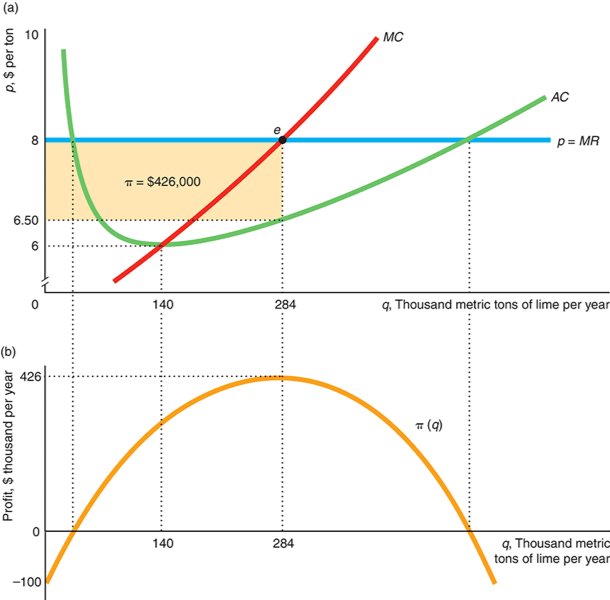
\includegraphics[scale=0.66]{../images/sr_profit.png}
	\end{figure}
}

\frame{
	\frametitle{Step two: Whether to produce}
	\begin{itemize}
		\item Recall: Firms should shut down in $R<VC$.
		\item[]
		\item For a competitive firm, this can be restated as: $p < AVC = VC/q$
		\item[]
		\item Three possible cases:
			\begin{enumerate}
			\item $p > AC$: Firm operates with a positive profit.
			\item $AC > p > AVC$: Firm operates with a negative profit.
			\item $AVC > p$: Firm shuts down.
			\end{enumerate}
		\end{itemize}
}

\frame{
	\frametitle{Step two: Whether to produce}
	\begin{figure}
	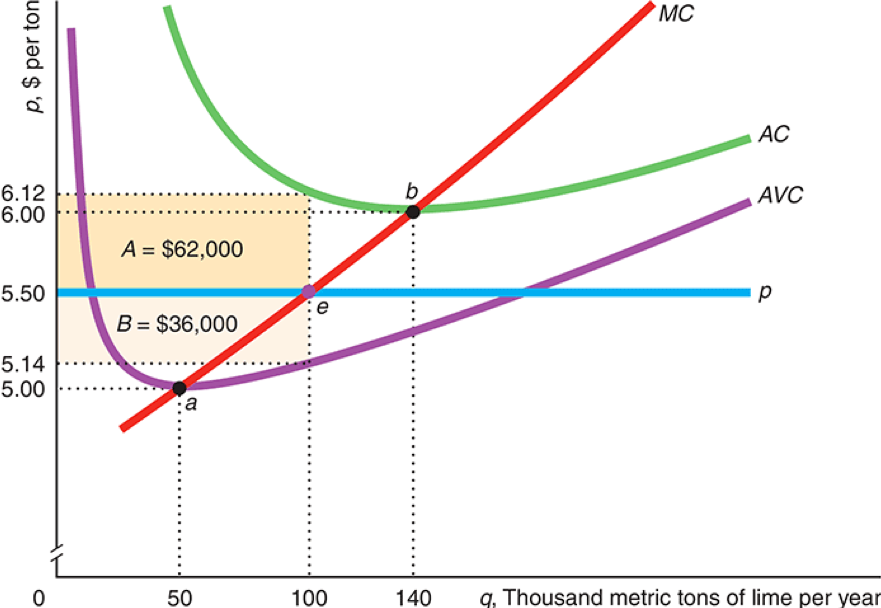
\includegraphics[scale=0.66]{../images/sr_shutdown.png}
	\end{figure}
}

\frame{
	\frametitle{Supply in the Short Run}
	\begin{itemize}
	\item We can use the shut-down rule to derive the firm's short run supply curve.
	\item[]
	\item If:
		\begin{itemize}
		\item $p \geq AVC$, firm produces such that $p=MC(q)$.
		\item $p < AVC$, the firm shuts down and produces nothing.
		\end{itemize}
	\item[]
	\item This means that a competitive firm's short run supply curve is its \textit{marginal cost curve above its minimum average variable cost}.
	\end{itemize}
}

\frame{
	\frametitle{Supply in the Short Run}
	\begin{figure}
	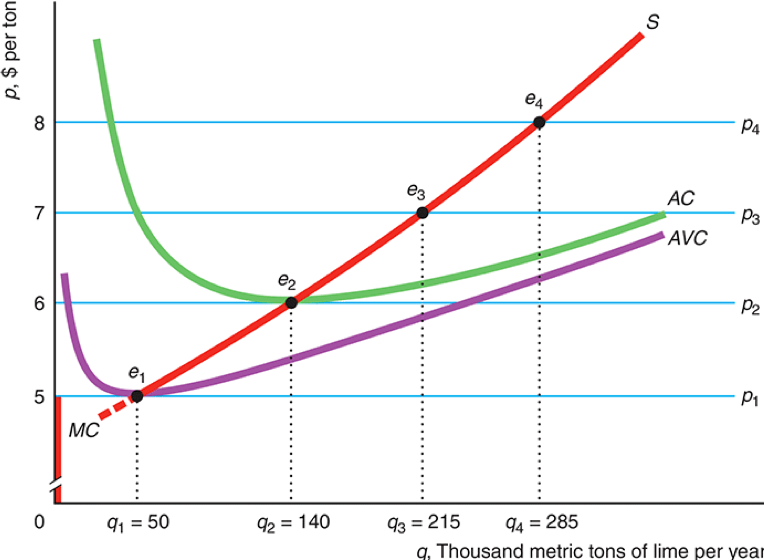
\includegraphics[scale=0.66]{../images/sr_supplycurve.png}
	\end{figure}
}

\frame{
	\frametitle{Market Supply in the Short Run}
	\begin{itemize}
	\item The short run market supply curve is given by the \underline{horizontal sum} of the supply curves of individual firms.
	\item[]
	\item The shape of the short run market supply curve depends on the extent of differences across firms.
	\end{itemize}
}

\frame{
	\frametitle{Market Supply in the Short Run}
	\begin{figure}
	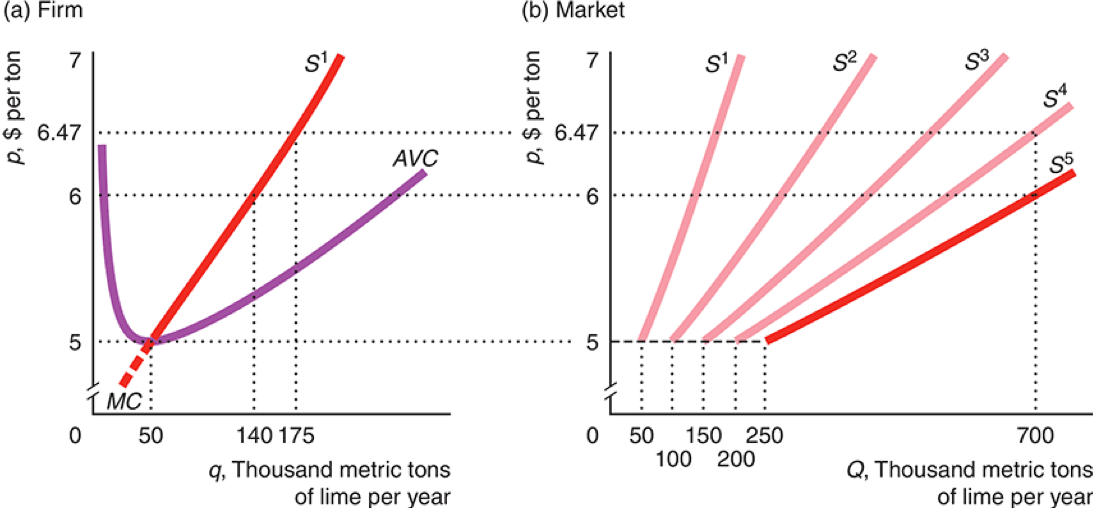
\includegraphics[scale=0.66]{../images/sr_mktsupply_identical.png}
	\caption{Market Supply with 5 Identical Firms}
	\end{figure}
}

\frame{
	\frametitle{Market Supply in the Short Run}
	\begin{figure}
	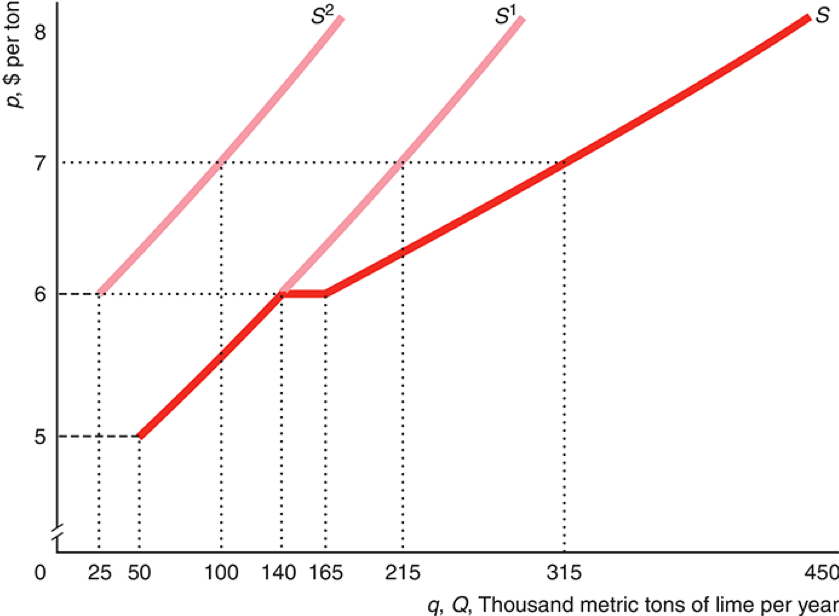
\includegraphics[scale=0.6]{../images/sr_mktsupply_diff.png}
	\caption{Market Supply with 2 Different Firms}
	\end{figure}
}


\frame{
	\frametitle{Oil Market Supply in the Short Run}
	\begin{figure}
	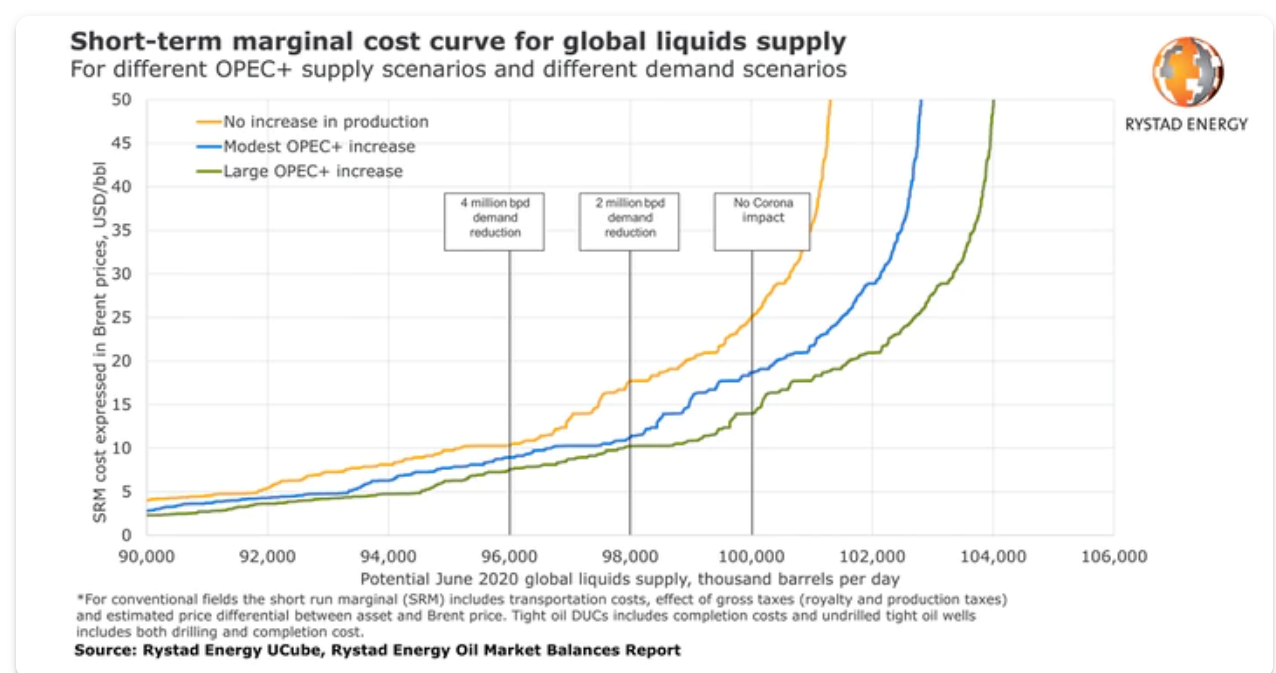
\includegraphics[scale=0.6]{../images/perfect_comp/rystad_short.png}
	%\caption{Market Supply with 2 Different Firms}
	\end{figure}
}



\frame{
	\frametitle{Equilibrium in the Short Run}
	\begin{itemize}
	\item We can determine the short-run competitive equilibrium by combining the short run market supply curve with the market demand curve.
	\item[]
	\item As an example, suppose there are five identical firms in the lime manufacturing industry.
	\end{itemize}
}

\frame{
	\frametitle{Equilibrium in the Short Run}
	\begin{figure}
	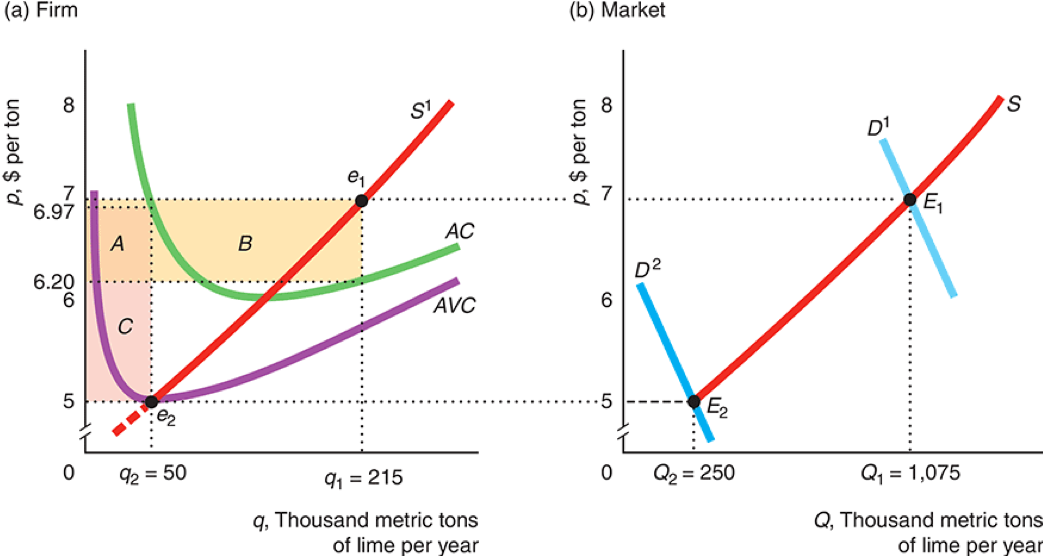
\includegraphics[scale=0.6]{../images/sr_eqm.png}
	\end{figure}
}

\frame{
	\frametitle{Outline}
	\begin{enumerate}
	\item Perfect Competition
	\item[]
	\item Competition in the Short Run
	\item[]
	\item \alert{Competition in the Long Run}
	\item[]
	\item Competition and Economic Well Being
	\end{enumerate}
}

\section{Competition in the Long Run}

\frame{
	\frametitle{Competition in the Long Run}
	\begin{itemize}
	\item Recall: In the long run, all inputs are variable.
	\item[]
	\item Production decisions again made to maximize profit via 2-step method.
	\item[]
	\item Key difference: long run shut down decision.
		\begin{itemize}
		\item In the long run, all costs are avoidable, so firm shuts down if it makes an economic loss by operating.
		\end{itemize}
	\end{itemize}
}

\frame{
	\frametitle{Shut Down Rule in the Long Run}
	\begin{itemize}
	\item We can again use the shut down rule to determine the supply curve.
	\item[]
	\item If:
		\begin{enumerate}
		\item $p \geq LRAC$: It is profit maximizing to operate.
		\item $p < LRAC$: It is profit maximizing to shut down.
		\end{enumerate}
	\item[]
	\item Thus, in the long run, the supply curve is \textit{the portion of the long-run marginal cost curve that lies above the minimum of the long-run average cost curve}.
	\end{itemize}
}

\frame{
	\frametitle{Supply in the Long Run}
	\begin{itemize}
	\item The long-run market supply curve is again the horizontal sum of the supply curves of the individual firms in the market.
	\item[]
	\item However, in the long run firms can enter or exit the market.
	\item[]
	\item Thus, to determine the long-run market supply curve, we need to determine how many firms will be in the market at each possible market price.
	\end{itemize}
}

\frame{
	\frametitle{Entry and Exit}
	\begin{itemize}
	\item The decision to enter or exit depends on whether a firm believes it can make a long-run profit.
	\item[]
	\item Any change in demand will lead to a change in the number of firms with free entry and exit.
		\begin{itemize}
		\item A rightward shift in the market demand curve attracts firms to enter the market until the last firm makes zero long run profit.
		\item A leftward shift in the market demand curve forces firms to exit the market until the last firm makes zero long run profit.
		\end{itemize}
	\end{itemize}
}

\frame{
	\frametitle{Long Run Supply Curve}
	\begin{itemize}
	\item The shape of the long-run market supply curve depends on:
		\begin{enumerate}
		\item Differences across firms.
		\item Ease of entry and exit.
		\end{enumerate}
	\item[]
	\item When firms can freely entry and exit the market, and all firms are identical, the long-run market supply curve is a \underline{horizontal line that intersects the minimum of the long-run average cost curve}.
	\end{itemize}
}

\frame{
	\frametitle{Long Run Supply Curve}
	\begin{figure}
	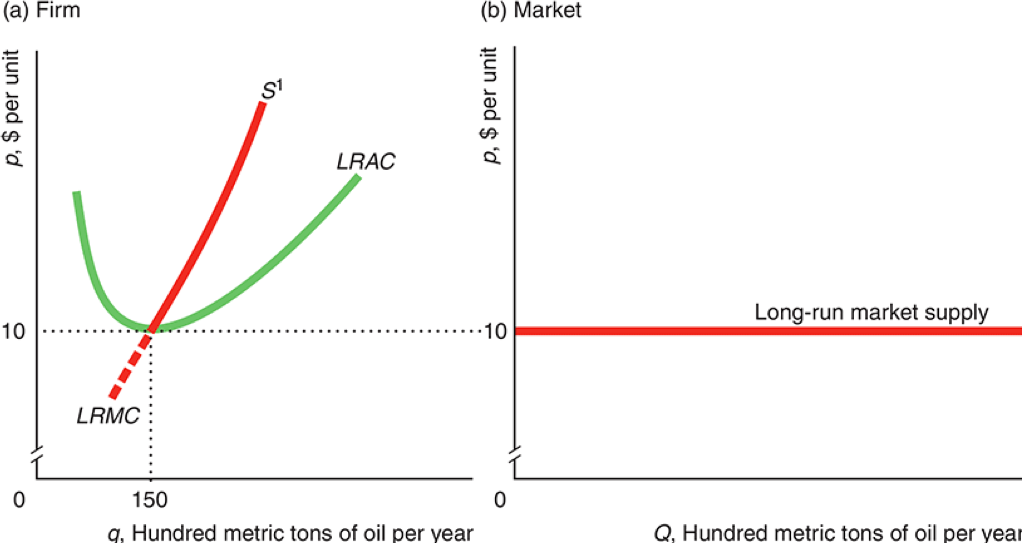
\includegraphics[scale=0.66]{../images/lr_identical.png}
	\end{figure}
}

\frame{
	\frametitle{Long Run Supply Curve}
	\begin{itemize}
	\item When entry is limited, but firms are identical, \textit{long-run market supply curves slope upward}.
		\begin{itemize}
		\item This can occur as a result of government restrictions, resource scarcity, or high entry costs.
		\end{itemize}
	\item[]
	\item When firms are not identical, \textit{long-run market supply curves can be upward sloping.}
		\begin{itemize}
		\item Firms with relatively low minimum average costs are willing to enter the market at low prices.
		\item If these firms cannot serve the entire market due to limited capacity/limited number, then firms with relatively high minimum average costs can enter, leading to an upward sloping supply curve.
		\end{itemize}
	\end{itemize}
}


\frame{
	\frametitle{Long Run Oil Supply Curve}
	\begin{figure}
	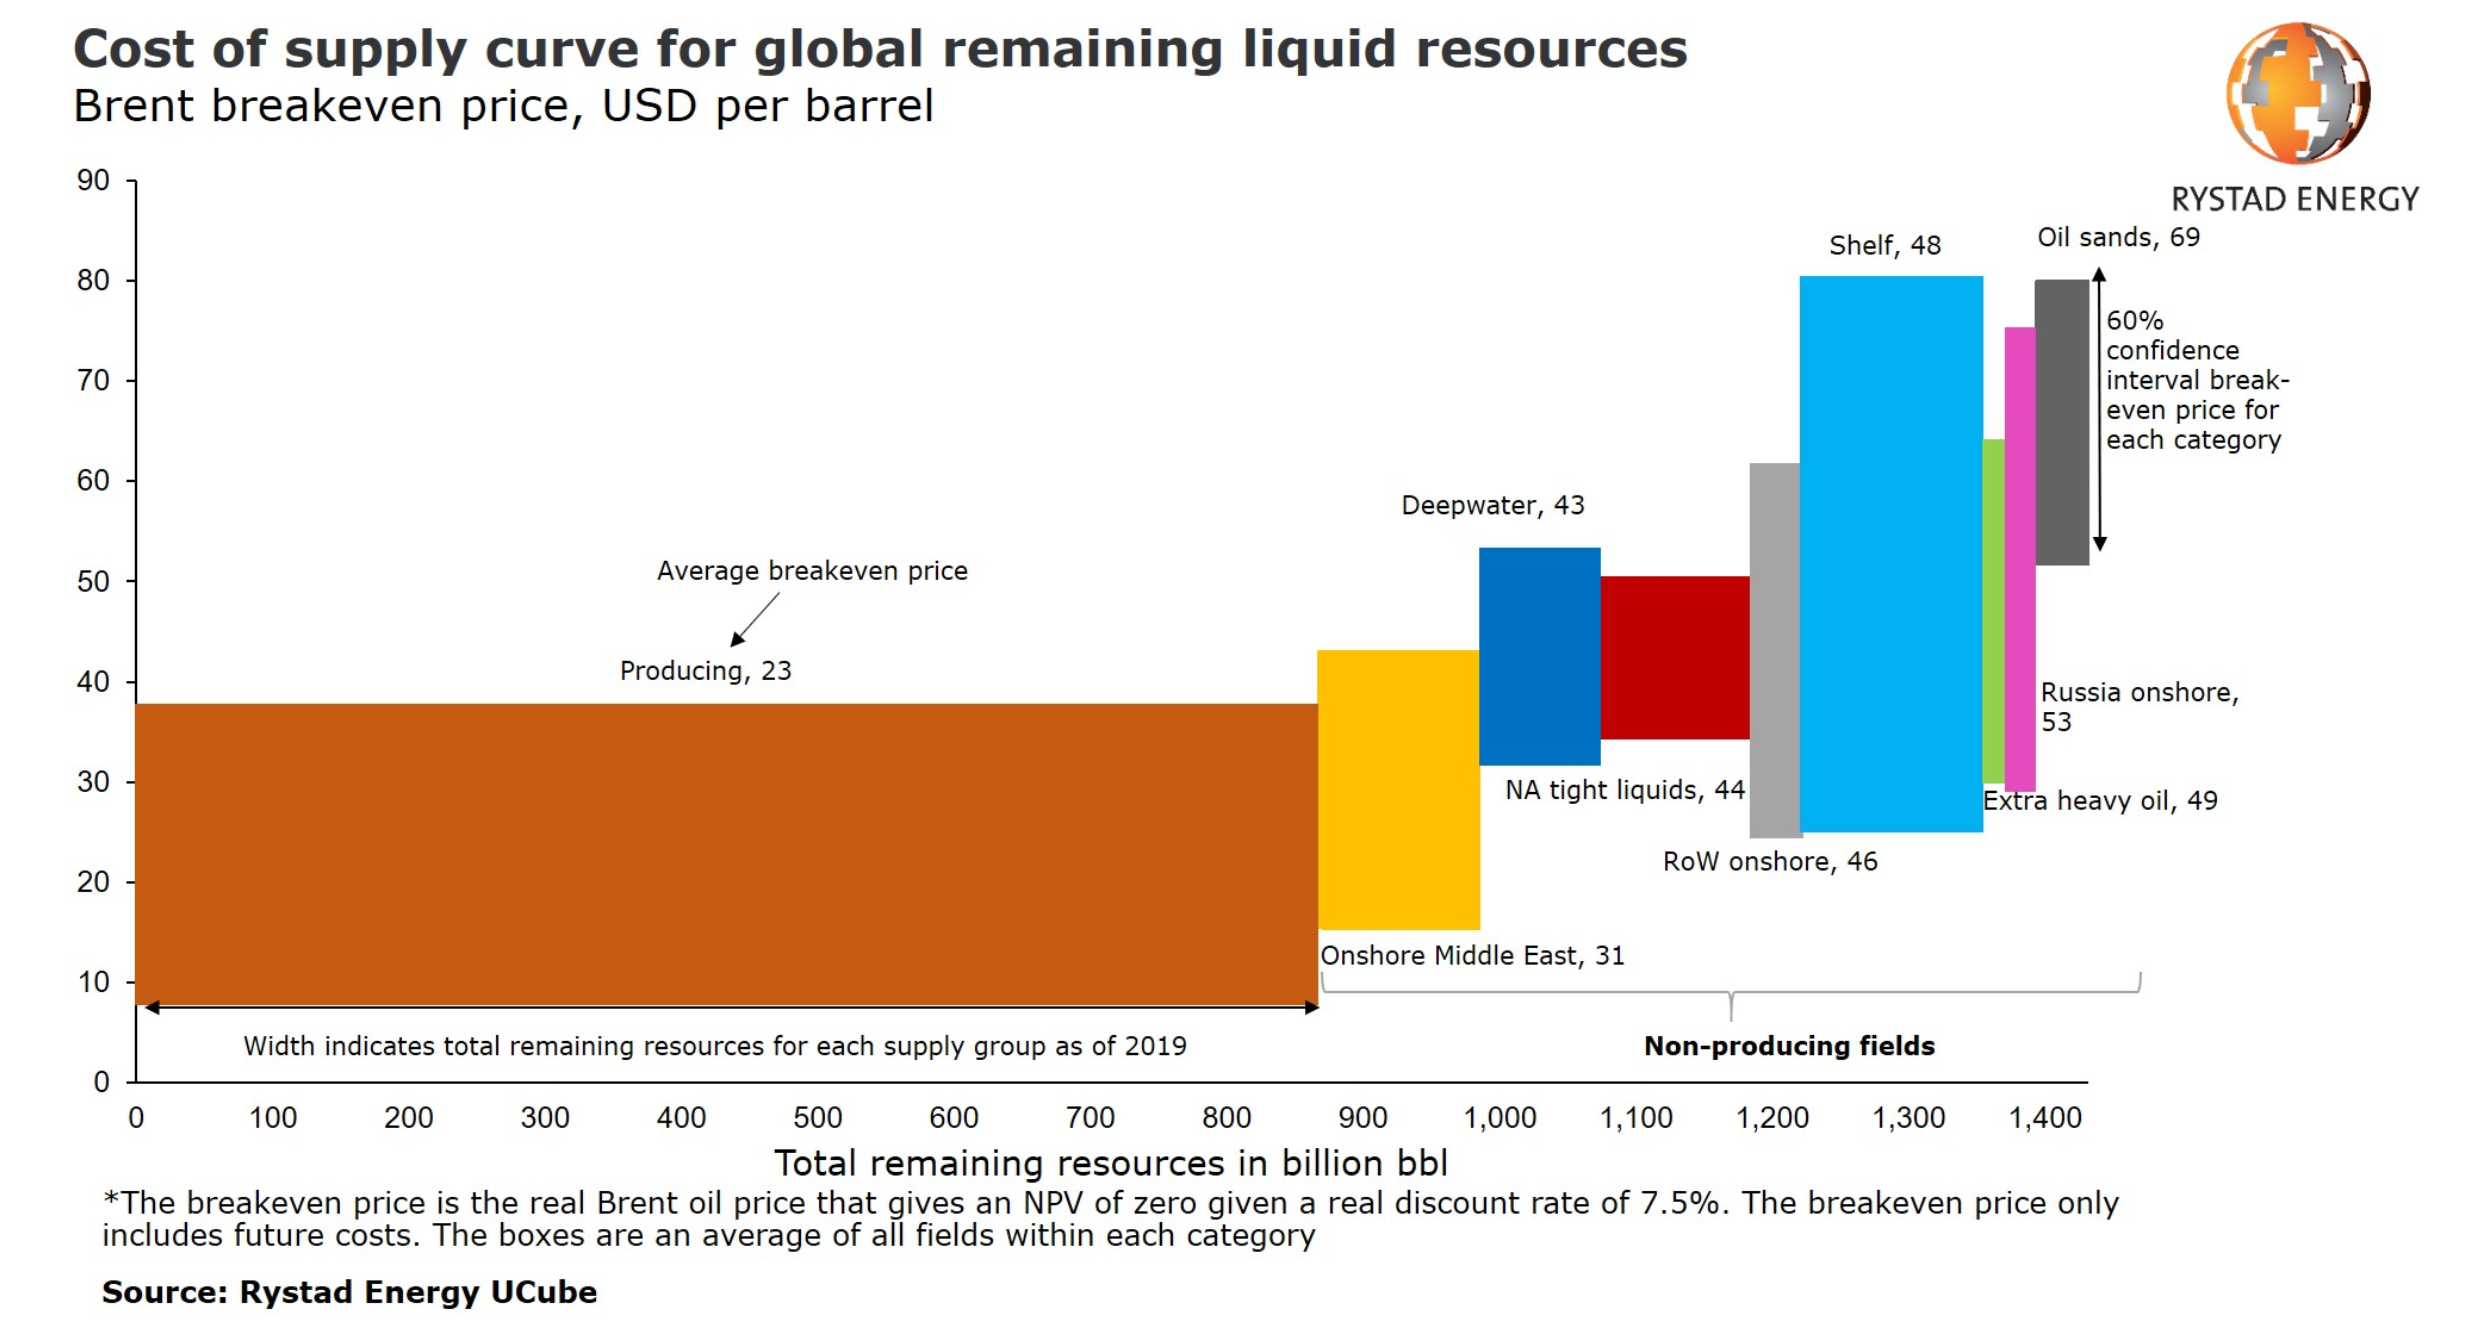
\includegraphics[scale=0.35]{../images/perfect_comp/rystad.png}
	\end{figure}
}


\frame{
	\frametitle{Long Run or Dynamic Equilibrium}
	\begin{itemize}
	\item The long-run competitive equilibrium occurs at the intersection of the long-run market supply and demand curves.
	\item[]
	\item With identical firms, constant input prices, and free entry and exit, the equilibrium price must equal the minimum long-run average cost.
	\item[]
	\item In this case, a shift in the demand curve only affects equilibrium quantity but not equilibrium price.
	\end{itemize}	
}

\frame{
	\frametitle{Long Run or Dynamic Equilibrium}
	\begin{figure}
	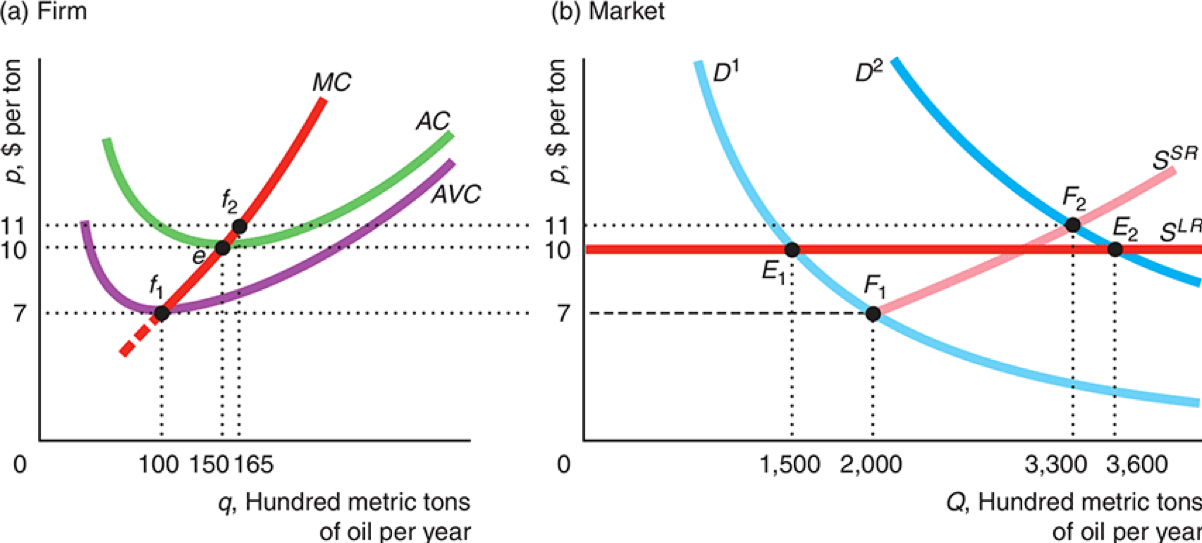
\includegraphics[scale=0.66]{../images/lr_eqm.png}
	\end{figure}
}

\frame{
	\frametitle{Long Run Equilibrium}
	\begin{itemize}
	\item The long-run market supply curve is horizontal if firms are free to enter and exit the market, firms have identical costs, and input prices are constant.
	\item[]
	\item In this case, all firms are operating at minimum long-run average cost.
	\item[]
	\item This means they are indifferent between shutting down and operating because they are earning zero economic profit.
	\item[]
	\item Key implication: \textbf{To survive in a competitive market in the long run, a firm must maximize its profit.}
		\begin{itemize}
		\item Firms that fail to maximize profit will be forced to exit.
		\end{itemize}
	\end{itemize}
}

\frame{
	\frametitle{Outline}
	\begin{enumerate}
	\item Perfect Competition
	\item[]
	\item Competition in the Short Run
	\item[]
	\item Competition in the Long Run
	\item[]
	\item \alert{Competition and Economic Well Being}
	\end{enumerate}
}

\section{Competition and Wellbeing}

\frame{
	\frametitle{Competition and Economic Wellbeing}
	\begin{itemize}
	\item The perfectly competitive model describes many aspects of the economy (agriculture, parts of the construction industry, some labor markets, much of retain and wholesale trade) very well.
	\item[]
	\item The model is also useful as a benchmark for understanding different industries.
	\item[]
	\item Why?
		\begin{itemize}
		\item Perfectly competitive markets maximize an important measure of economic well being: \underline{total surplus}.
		\end{itemize}
	\end{itemize}
}

\frame{
	\frametitle{Total Surplus}
	\begin{itemize}
	\item \underline{Total Surplus} (TS) is a monetary measure of the total benefit to all market participants from market transactions.
		\begin{itemize}
		\item It is a measure of the \textit{gains from trade}.
		\end{itemize}
	\item[]
	\item Total surplus depends on:
		\begin{itemize}
		\item The gains for consumers (\textit{consumer surplus}).
		\item The gains for producers (\textit{producer surplus}).
		\end{itemize}
	\end{itemize}
}

\frame{
	\frametitle{Consumer Surplus}
	\begin{itemize}
	\item \underline{Consumer Surplus} (CS) is the monetary difference between what a consumer is \textit{willing to pay} for the quantity of good purchased and what the consumer actually pays.
		\begin{itemize}
		\item This is the dollar value of gains from trade for the consumer.
		\end{itemize}
	\item[]
	\item The demand curve reflects a consumer's \underline{marginal willingness to pay}.
		\begin{itemize}
		\item The demand curve reflects the maximum amount a consumer will spend for an extra unit.
		\end{itemize}
	\item[]
	\item This means we can measure consumer surplus as the area below the demand curve and above the market price up to the quantity actually consumed.
	\end{itemize}
}

\frame{
	\frametitle{Consumer Surplus}
	\begin{figure}
	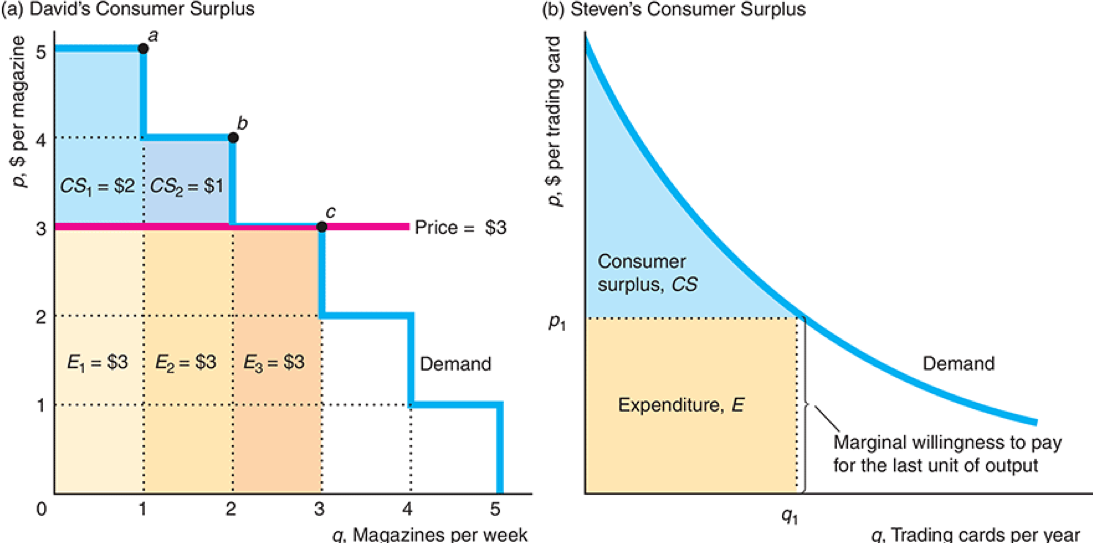
\includegraphics[scale=0.66]{../images/cs_steps.png}
	\end{figure}
}

\frame{
	\frametitle{Consumer Surplus}
	\begin{figure}
	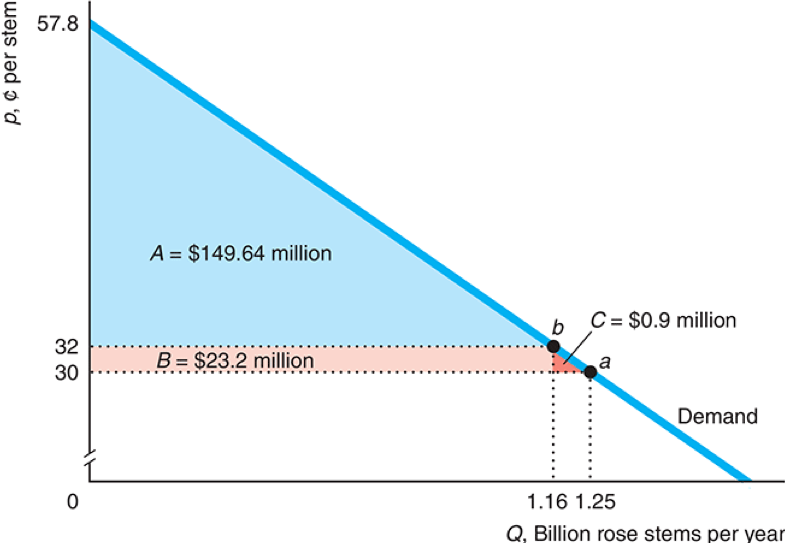
\includegraphics[scale=0.66]{../images/cs_smooth.png}
	\end{figure}
}

\frame{
	\frametitle{Producer Surplus}
	\begin{itemize}
	\item \underline{Producer Surplus} is the monetary difference between the amount a good sells for, and the minimum amount necessary for the producers to be \textit{willing to produce} the good.
		\begin{itemize}
		\item This is the dollar value of gains from trade for the producer.
		\end{itemize}
	\item[]
	\item Producer surplus is the area above the supply curve and below the market price up to the quantity actually demanded.
	\end{itemize}
}

\frame{
	\frametitle{Producer Surplus}
	\begin{figure}
	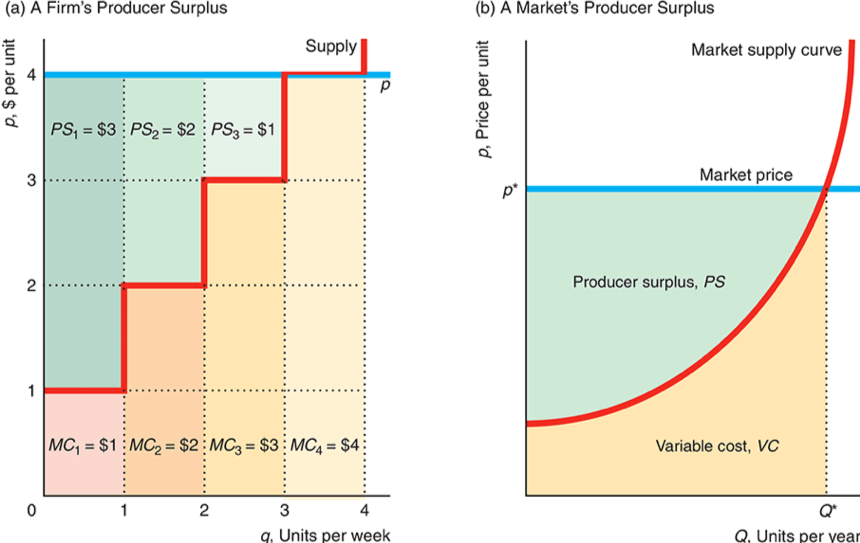
\includegraphics[scale=0.66]{../images/ps_steps.png}
	\end{figure}
}

\frame{
	\frametitle{Total Surplus}
	\begin{itemize}
	\item By definition, total surplus is the sum of consumer surplus and producer surplus.
	\item[]
	\item \textit{Perfect competition maximizes total surplus. Producing less or more than the competitive level of output lowers total surplus.}
	\end{itemize}
}

\frame{
	\frametitle{Equilibrium}
	\begin{figure}
	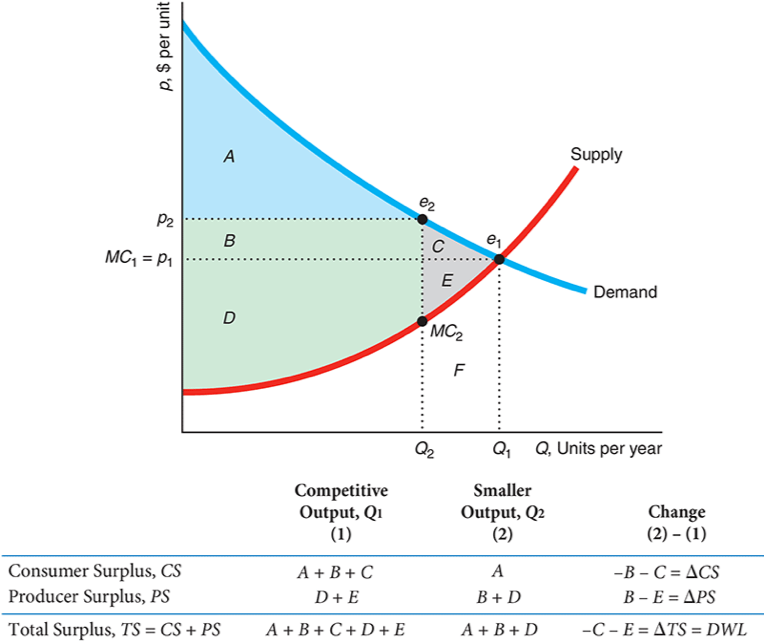
\includegraphics[scale=0.66]{../images/ts_eqm.png}
	\end{figure}
}

\frame{
	\frametitle{Deadweight Loss}
	\begin{definition}[Deadweight Loss]
	The net reduction in total surplus from a loss in surplus by one group that is not offset by a gain in surplus by another group from an action that alters a market equilibrium.
	\end{definition}
}

\frame{
	\frametitle{Deadweight Loss}
	\begin{itemize}
	\item Any government policy that limits trade in a competitive market reduces total surplus.
	\item[]
	\item The reduction in total surplus is the deadweight loss created by the policy.
	\item[]
	\item Example: The effects of a price ceiling.
	\end{itemize}
}

\frame{
	\frametitle{Don't listen to David Suzuki!}
	\begin{itemize}
	\item \underline{Important caveat}: While government intervention reduces economic wellbeing when markets are perfectly competitive, \textbf{THIS IS NOT TRUE IN GENERAL!}
	\item[]
	\item \textit{Government intervention may increase well-being in non-competitive markets, such as in a monopoly.}
	\end{itemize}	
}

\section{Takeaways}

\frame{
	\frametitle{Takeaways}
	\begin{enumerate}
	\item Perfect competition is characterized by price taking.
	\item[]
	\item With perfect competition:
		\begin{itemize}
		\item Firms operate in the short run if price is above average variable cost, and the market equilibrium is determined by the intersection of demand and the short-run market supply curve.
		\item Firms operate in the long run if price is above long-run average cost, and the market equilibrium is determined by the intersection of demand and the long-run market supply curve.
		\end{itemize}
	\item[]
	\item Perfect competition maximizes total surplus.
	\end{enumerate}
}

\end{document}
